%%%%%%%%%%%%%%%%%%%%%%%%%%%%%%%%%%%%%%%%%%%%%%%%%%%%%%%%%%%%%%%%%%%%%%%%%%%%%%%%
% DEFINE DOCUMENT TYPE
%%%%%%%%%%%%%%%%%%%%%%%%%%%%%%%%%%%%%%%%%%%%%%%%%%%%%%%%%%%%%%%%%%%%%%%%%%%%%%%%
\documentclass[11pt, oneside]{mnthesis}


%%%%%%%%%%%%%%%%%%%%%%%%%%%%%%%%%%%%%%%%%%%%%%%%%%%%%%%%%%%%%%%%%%%%%%%%%%%%%%%%
% IMPORT PACKAGES
%%%%%%%%%%%%%%%%%%%%%%%%%%%%%%%%%%%%%%%%%%%%%%%%%%%%%%%%%%%%%%%%%%%%%%%%%%%%%%%%
\usepackage{epic,eepic,units}
\usepackage{hyperref}
\usepackage{array}
\usepackage{longtable}
\usepackage{mathrsfs}
\usepackage{multirow}
\usepackage{bigstrut}
\usepackage{cite}
\usepackage{paralist}
\usepackage[stable]{footmisc}   %Lets us use footnotes in section headers.
% \usepackage[style={square, numbers}]{natbib}
\usepackage{listings, multicol}
\usepackage{subcaption}  % subfigures
\usepackage{bibentry}
\usepackage{makeidx}
\usepackage{tabularx,colortbl}
\usepackage[dvipsnames]{xcolor}
\usepackage{flushend}
\usepackage{cite}
\usepackage{amsmath}
\usepackage{amssymb}
\usepackage{epsfig}
\usepackage{stmaryrd}
\usepackage{url}
\usepackage{amsmath}
\usepackage{bm}
\usepackage{amsthm}
\usepackage{amssymb}
\usepackage{multirow}
\usepackage{latexsym}
\usepackage{graphics}
\usepackage{graphicx}
\usepackage{enumitem}
\usepackage{comment}
\usepackage{longtable}
\usepackage{supertabular}
\usepackage{times}
\usepackage{listings}
%\usepackage{subfigure}
\usepackage{color}
\usepackage{booktabs}
\usepackage{balance}
\usepackage{xspace}
\usepackage[ruled, vlined, linesnumbered]{algorithm2e}
\usepackage[autostyle]{csquotes}
\usepackage[]{algorithm2e}
\usepackage{authblk}
\newcolumntype{L}[1]{>{\raggedright\let\newline\\\arraybackslash\hspace{0pt}}p{#1}}
\newcolumntype{C}[1]{>{\centering\let\newline\\\arraybackslash\hspace{0pt}}p{#1}}
\newcolumntype{R}[1]{>{\raggedleft\let\newline\\\arraybackslash\hspace{0pt}}p{#1}}
\newtheorem{theorem}{Theorem}
\newtheorem{definition}{Definition}
\newcommand{\mkeyword}[1]{\mbox{\texttt{#1}}}
\DeclareMathOperator{\kuop}{uop}
\DeclareMathOperator{\kbop}{bop}
\DeclareMathOperator{\kite}{ite}
\DeclareMathOperator{\kpre}{pre}
\DeclareMathOperator{\dom}{dom}
\DeclareMathOperator{\ktrue}{true}
\DeclareMathOperator{\kfalse}{false}
\DeclareMathOperator{\kselect}{select}
\DeclareMathOperator{\ran}{range}
\newcommand{\lbb}{[\![}
\newcommand{\rbb}{]\!]}
\newcommand{\expr}{\phi}
\newcommand{\exprS}{\Phi}
\newcommand{\danielle}[1]{\textcolor{blue}{#1}}

%Dealing with dutch names:
% http://tex.stackexchange.com/questions/40747/bibtex-handling-of-the-dutch-van-name-prefix-with-natbib
\DeclareRobustCommand{\VAN}[2]{#2}



%%%%%%%%%%%%%%%%%%%%%%%%%%%%%%%%%%%%%%%%%%%%%%%%%%%%%%%%%%%%%%%%%%%%%%%%%%%%%%%%
% ADDITIONAL PREABLE MATERIAL
%%%%%%%%%%%%%%%%%%%%%%%%%%%%%%%%%%%%%%%%%%%%%%%%%%%%%%%%%%%%%%%%%%%%%%%%%%%%%%%%
\hypersetup{
    colorlinks,
%     %Set the link colors.
%     citecolor=black,
%     filecolor=blue,
%     linkcolor=blue,
%     urlcolor=blue
    %To turn off color, comment out the block above and uncomment the block
    % below.
    citecolor=black,
    filecolor=black,
    linkcolor=black,
    urlcolor=black
}


% Suppresses inline citation page numbers if they are defined using \cite.
    \let\oldcite\cite
    \renewcommand\cite[2][]{\oldcite{#2}}

% \setcounter{secnumdepth}{5}

% % \appendix{Glossary}
% \begin{description}
% \item[process]\label{def:process}  ``set of interrelated or interacting
%     activities which transforms inputs into outputs''~\cite{_iso9000_2005}
% \item[work package]\label{def:work_package}  small pieces of functionality or
%     supporting documentation to be completed
% \end{description}

\newglossaryentry{def:brownfield_project}
{
    name={brownfield project},
    description={a project that is based on or must coexist with one or more
            legacy systems} 
}

\newglossaryentry{def:challenged_project}
{
    name={challenged project},
    description={a project that completes ``late, over-budget, and/or with less
            than required features or functions''~\cite[p.1]{_chaos_2013}; with
            agile techniques, typically only schedule and cost concerns are
            measured} 
}


\newglossaryentry{def:failed_project}
{
    name={failed project},
    description={a project that was unable to complete because it was 
        ``cancelled prior to completion or delivered and never 
        used''~\cite[p.1]{_chaos_2013}} 
}


\newglossaryentry{def:greenfield_project}
{
    name={greenfield project},
    description={a project that is not constrained by any prior work, such as
            legacy systems} 
}

\newglossaryentry{def:method-family}
{
    name={method-family},
    description={the process type; a group of processes that can be
        characterized by a set of well-defined properties (e.g., agile,
        traditional)},
    plural={method-families}
}


\newglossaryentry{def:oracle}
{
    name={oracle},
    description={the standard by which we can compare the output of a
        system being evaluated} 
}


\newglossaryentry{def:process}
{
    name=process,
    description={``set of interrelated or interacting
                activities which transforms inputs into
                outputs''~\cite{_iso9000_2005}},
    user1={_iso9000_2005},
    plural=processes 
}


\newglossaryentry{def:process_characterization}
{
    name={process characterization},
    description={determining the properties of the project and product to be
        completed and establishing the project's goals (such as focusing on
        quality)~\cite{xu_using_2008}}
}


\newglossaryentry{def:process_model}
{
    name={process model},
    description={an abstraction of a process; this may be either a model that
        represents a concrete process or a pre-tailored form of a model (e.g.,
        scrum, extreme programming, spiral model)}
}


\newglossaryentry{def:project_network}
{
    name={project network},
    description={the set of \glspl{def:work_package} and their
        interdependencies}
}


\newglossaryentry{def:successful_project}
{
    name={successful project},
    description={a completed project that was ``delivered on time, on budget,  
        with required features and functions''~\cite[p.1]{_chaos_2013}}
}


\newglossaryentry{def:triple_constraint}
{
    name={triple-constraint},
    description={a set of metrics---cost, schedule, and scope (including
        quality)---commonly used to evaluate project success; also a method for
        balancing project priorities (limiting one of the metrics results in
        changes---increased cost, increased schedule, and decreased scope---in
        one or both of the other constraints)} 
}


\newglossaryentry{def:work_breakdown_structure}
{
    name={work breakdown structure},
    description={}
}


\newglossaryentry{def:work_package}
{
    name={work package},
    description={small pieces of functionality or supporting documentation to be
                 completed}
}





% 
% 
%     \item[High-level Process Model Selection]  Select the high-level process
%             model (e.g. Scrum or XP for the agile method-family) as the basis
%             for further specialization.
%     \item[Tailoring]  Adapting the process model to meet the
%             specific needs or constraints of the organization, product, and
%             project.
%     \item[Process Evaluation (Verification and Validation)]  Verifying and
%         validating that the process (or process model instance) meets the needs
%         of the team and is ``consistent with the project goals and
%         environment''~\cite{xu_using_2008}.  This can be performed in a number
%         of ways.
%             \textbf{TODO -- this part should be its own (sub)section.}
%     \item[Adoption (Execution)]  Implementing the process within the
%             organization to complete the project.  Depending on the process,
%             this may involve \textit{in~situ} process analysis and improvements.
%     \item[Post-mortem Analysis]  Evaluating the process after it has been
%             executed to improve later projects.
% \makeglossaries

% %%%%%%%%%%%%%%%%%%%%%%%%%%%%%%%%%%%%%%%%%%%%%%%%%%%%%%%%%%%%%%%%%%%%%%%%%%%%%%%%
% Custom definitions
%%%%%%%%%%%%%%%%%%%%%%%%%%%%%%%%%%%%%%%%%%%%%%%%%%%%%%%%%%%%%%%%%%%%%%%%%%%%%%%%
\newcommand{\C}{{\mathrm{c}}}

\newcommand{\COS}{{\mathrm{cos}}}
\newcommand{\SIN}{{\mathrm{sin}}}
\newcommand{\DOF}{{\mathrm{dof}}}
\newcommand{\MSEC}{\mu{\mathrm{s}}}
\newcommand{\NS}{\mathrm{ns}}
\newcommand{\PPM}{{\mathrm{ppm}}}
\newcommand{\ENR}{{\mathrm{GeV}}}
\newcommand{\MOM}{{\mathrm{GeV/c}}}

\newcommand{\CONT}{\noindent}
\newcommand{\FIG}{Fig.\ }
\newcommand{\FIGS}{Figs.\ }
\newcommand{\SEC}{Sec.\ }
\newcommand{\SECS}{Secs.\ }
\newcommand{\TAB}{Table }
\newcommand{\TABS}{Tables }
\newcommand{\EQ}{Eq.\ }
\newcommand{\EQS}{Eqs.\ }
\newcommand{\APP}{Appendix }
\newcommand{\APPS}{Appendices }
\newcommand{\CHP}{Chapter }
\newcommand{\CHPS}{Chapters }

\newcommand{\OFF}{\emph{G2off}~}
\newcommand{\TOO}{\emph{G2Too}~}
%%%%%%%%%%%%%%%%%%%%%%%%%%%%%%%%%%%%%%%%%%%%%%%%%%%%%%%%%%%%%%%%%%%%%%%%%%%%%%%%


% FROM:
% http://tex.stackexchange.com/questions/4297/how-to-place-a-full-citation-in-the-abstract-using-bibtex
% \newcommand{\ignore}[1]{}
% \newcommand{\nobibentry}[1]{{\let\nocite\ignore\bibentry{#1}}}
% % apsrev entries in the text need definitions of these commands
% \newcommand{\bibfnamefont}[1]{#1}
% \newcommand{\bibnamefont}[1]{#1}
\nobibliography*

%%%%%%%%%%%%%%%%%%%%%%%%%%%%%%%%%%%%%%%%%%%%%%%%%%%%%%%%%%%%%%%%%%%%%%%%%%%%%%%%
% STRUCTURE SET-UP
%%%%%%%%%%%%%%%%%%%%%%%%%%%%%%%%%%%%%%%%%%%%%%%%%%%%%%%%%%%%%%%%%%%%%%%%%%%%%%%%
\newcommand{\apriori}{\textit{a~priori} }
\newcommand{\Apriori}{\textit{A~priori} }


% Change the line spacing!
\linespread{1}

%%%%%%%%%%%%%%%%%%%%%%%%%%%%%%%%%%%%%%%%%%%%%%%%%%%%%%%%%%%%%%%%%%%%%%%%%%%%%%%%
% BEGIN DOCUMENT
%%%%%%%%%%%%%%%%%%%%%%%%%%%%%%%%%%%%%%%%%%%%%%%%%%%%%%%%%%%%%%%%%%%%%%%%%%%%%%%%
\begin{document}

%%%%%%%%%%%%%%%%%%%%%%%%%%%%%%%%%%%%%%%%%%%%%%%%%%%%%%%%%%%%%%%%%%%%%%%%%%%%%%%%
% title.tex - Set up the beginning of thesis.
%%%%%%%%%%%%%%%%%%%%%%%%%%%%%%%%%%%%%%%%%%%%%%%%%%%%%%%%%%%%%%%%%%%%%%%%%%%%%%%%
% For a  PhD give the command \phd. Default is masters
%\degree (normally Doctor of Philosophy or Master of Science)
%\initials (normally Ph.D. or M.S.)
%\ms % use if for a Master of Science thesis
\phd % use if for a Ph.D. dissertation
% \draft
%\topicProposaltrue

\title{\textbf{Architectural Modeling and Analysis for Safety Engineering}}
\author{Danielle Stewart}
\campus{University of Minnesota} 
\program{Computer Science and Engineering} 
% \degree{Doctor of Philosophy}
\director{Prof. Mats P. E. Heimdahl and Dr. Michael W. Whalen} 

% Optionally specify the month and year.
\submissionmonth{August} % defaults to current month.
\submissionyear{2020} % defaults to current year.

%Comment out below on final copy
\abstract{Model-based development tools are increasingly being used for system-level development of safety-critical systems. Architectural and behavioral models  provide important information that can be leveraged to improve the system safety analysis process. Model-based design artifacts produced in early stage development activities can be used to perform system safety analysis, reducing costs and providing accurate results throughout the system life-cycle.

Safety analysis is used to ensure that critical systems operate within some level of safety when failures are present. As critical systems become more dependent on software components, it becomes more challenging for safety analysts to comprehensively enumerate all possible failure causation paths. Any automated analyses should be sound to sufficiently prove that the system operates within the designated level of safety. This paper presents a compositional approach to the generation of fault forests (sets of fault trees) and minimal cut sets. We use a behavioral fault model to explore how errors may lead to a failure condition. The analysis is performed per layer of the architecture and the results are automatically composed. A complete formalization is given. We implement this by leveraging minimal inductive validity cores produced by an infinite state model checker. This research provides a sound alternative to a monolithic framework. This enables safety analysts to get a comprehensive enumeration of all applicable fault combinations using a compositional approach to generate while generating artifacts required for certification.


%The result is an extension to the Architecture Analysis and Design Language (AADL) that supports modeling of system behavior under failure conditions. This \emph{Safety Annex} enables the independent modeling of component failures and allows safety engineers to weave various types of fault behavior into the nominal system model. The accompanying tool support uses model checking to propagate errors from their source to their effect on safety properties without the need to add separate propagation specifications. 



}
\words{331}    % number of words in the abstract
\copyrightpage % Do you want copyright protection?
\acknowledgements{
Acknowledgements are tricky to write and usually left unread. I will make this quick and painless for anyone who wishes to read it. \\

Thank you to my advisors Mats and Mike, and committee members Darren, Antonia, and John. I couldn't have done this without your support.

My grandmother, Patricia. You taught me to search for knowledge.  My never ending questions were always met with: ``look it up." You encouraged my intellect in ways no one else did. And finally, my wonderful brother Josiah and Alex. I would not have made it to today without you both. Thank you. Really. 

}
%\dedication{To my Grandfather, Leal:% I survived you. You did your very best to ruin me, but you failed. You simultaneously did your best to raise me to be an intelligent, wise, and truthful woman. This you succeeded in. 

% It was a strange moment when after months of struggle, the committee made your birthday my day of defense. It was perfectly fitting---one of those synchronous moments that seem to follow me. Another was the day I got my first horse, Nicholas. That was also on your birthday. 

% The cruelest and darkest moments of my life, you saw. You were there and you created them. You almost killed me in more ways than one. But here I am. People have said that I am not who I am because of you, but I know they are wrong. You helped shaped me into me. If I could go back in time and make it all different, I couldn't... it would be suicide. I would be fundamentally different. And I like who I am. I like what came of that mess. 

% Yet at the same time, I wish things could have been different. I wish you would have been a good grandfather. You are the monster under my bed and I will love you for the rest of my life. Strange, isn't it. 

% This work is for you. I close the page on this chapter of my life, but never on the chapter of you. You weave your way through my every day and that is okay. You are part of me. }

% Use a special preface
%\extra{\chapter*{Author Declaration}
 \addcontentsline{toc}{chapter}{Author Declaration}
Some of the material presented within has previously been published in the
following papers:

\begin{itemize}
  \item \bibentry{stewart2020safety}
  \item \bibentry{nasaFinalReport}
  \item \bibentry{SATechReport}
  \item \bibentry{Stewart17:IMBSA}
\end{itemize}

\flushleft
All the work contained within represents the original contribution of the
author.}

% The \beforepreface command actually causes insertion of the title, 
% abstract, signature, and copyright pages into the new document.
\beforepreface 

% Define the text to go before the table of contents
\figurespage
\tablespage

% The \afterpreface command actually causes insertion of the
% contents, list of figures, etc. into the new document.
\afterpreface            
%%%%%%%%%%%%%%%%%%%%%%%%%%%%%%%%%%%%%%%%%%%%%%%%%%%%%%%%%%%%%%%%%%%%%%%%%%%%%%%%





%%%%%%%%%%%%%%%%%%%%%%%%%%%%%%%%%%%%%%%%%%%%%%%%%%%%%%%%%%%%%%%%%%%%%%%%%%%%%%%%
% CONTENT
%%%%%%%%%%%%%%%%%%%%%%%%%%%%%%%%%%%%%%%%%%%%%%%%%%%%%%%%%%%%%%%%%%%%%%%%%%%%%%%%
% Input the sectons here using \input{fileName}
%%%


\chapter{Introduction}
\label{chap:intro}
In our increasingly computerized world, the concept of system safety has become of great importance to many different fields. A \emph{complex safety critical system} is one whose safety cannot be shown only through testing, whose logic is difficult to comprehend without the aid of analytical tools, and that may contribute -- directly or indirectly -- to loss of life, damage of the environment, or large economic losses~\cite{SAE}. Critical systems can be found for example in the aviation, automotive, nuclear, or medical industries, and the process of designing such systems, from inception to deployment in society, presents numerous problems with which researchers have been contending. 

System safety has been an important factor in the design of systems for many years, but the birth of system safety as we know it today began shortly after World War II. The US Air Force was having numerous aircraft accidents; over 7,700 aircraft were lost between the years of 1952 and 1966 and over 8,000 people were killed~\cite{hammer}. Their approach to aircraft system safety was to analyze the accident and ``fix" the problem for the next flight. At the time, many of the accidents were blamed on pilots, but a number of flight engineers did not believe the causes were so simple. They posited that safety must be designed and built into the aircraft~\cite{levesonWhitePaper}. With the growth of nuclear capabilities, the defense industry complex, and the overall increase of computerization, the need to abandon a ``fly-fix-fly" approach to safety was imminent~\cite{miller1954applying, levesonWhitePaper, hammer}. The goal became to avoid accidents, instead of fixing a problem after an accident occurs.

Today, system safety analysis is crucial in the development life cycle of critical systems to ensure adequate safety as well as demonstrate compliance with applicable standards. The process meant to guide the development and certification of safety critical systems has been standardized by competent authorities~\cite{SAE,SAE:ARP4761,SAE:ARP4754A}.

A prerequisite for any safety analysis is a thorough understanding of the system architecture and the behavior of its components; safety engineers use this understanding to explore the overall system behavior, assess the effect of failures on the system's safety objectives, and construct the accompanying safety analysis artifacts so that safe operation can be ensured and demonstrated~\cite{SAE:ARP4761,SAE:ARP4754A}. System information and safety artifacts can also reveal missing requirements or be used to strengthen the existing ones, and they give crucial information about how the system responds to faulty components or errors in functionality that cross component boundaries~\cite{Bozzano:2010:DSA:1951720}.  An important goal of the safety assessment process is to show what kinds of failures may occur during normal use of the system. These analyses, both qualitative and quantitative, can provide information on how the system is safe (or unsafe) for use~\cite{roland1990system}.

The development life cycle of critical systems can be roughly seen as two main thrusts that occur in tandem: one side focuses on the system development itself; the hardware and software design, the requirements of the system, and the logical behavior of the components and their interactions. The other side is safety assessment of the system. Safety analysts are concerned with the failure of a system; systems can be unsafe (fail) with or without component or software failures. Safety analysts use information generated during the system design and development process and analyze the system from the perspective of failure; in other words, they focus on what can make the system unsafe. This is used to strengthen the system design and provide feedback into the development process.

Due to the complex nature of this arrangement, these sides are in reality not always done in strict parallel and are rarely synchronized perfectly. Furthermore, the artifacts given to safety analysts from system engineers are not always formal in nature, they may come from various sources, and they often do not clearly define the entire system and its behavior. To address this concern, \emph{model-based system engineering} (MBSE) and \emph{model-based safety assessment} (MBSA) caught the attention of researchers in the safety critical system domains~\cite{Joshi05:Dasc,CAV2015:BoCiGrMa,info17:HaLuHo,5979344,Gudemann:2010:FQQ:1909626.1909813}. In model-based engineering, the development efforts are centered on a model of the intended system. Various techniques, such as formal verification, testing, test case generation, execution and animation, etc., can be used to validate and verify the proposed system behavior. Given this increase in model-based development in critical systems, leveraging the resultant models in the safety analysis process and automating the generation of safety analysis artifacts holds great promise in terms of accuracy and efficiency. 

Many of the techniques proposed for MBSA require the development of {\em fault models} specific for safety analysis; that is, the techniques do not rely on the \emph{extension} of existing system models, but rather require purpose-built fault models that are separate entities~\cite{symbAltaRica, DBLP:conf/tacas/BittnerBCCGGMMZ16, info8010007, Gudemann:2010:FQQ:1909626.1909813}. Thus there is a system model used by the system engineers and a fault model used by safety analysts. %It requires extra manual labor to create a separate fault model that accurately describes the system model itself. 
As systems become more complex, it becomes difficult to ensure that the fault model developed for safety analysis conforms with the the model created for the development efforts -- just as it is difficult to show that the system model conforms to the actual implemented system. Another problem of this approach is that any changes made in system development are not automatically reflected in the safety analysis process; those changes must be communicated to safety analysts and incorporated into the separate fault model. This brings us right back to a non-model based approach.

Part of the safety assessment process determines how faults can manifest themselves in a particular component, but also how a manifested fault (or \emph{error}) can propagate through a system. Error propagation can be handled a variety of ways; most commonly this is done through the use of signal flow diagrams, a deep understanding of the system components, and the intuition of a good analyst~\cite{lisagor2010failure}. Various research has attempted to address this gap by providing tools that operate over a model and provide some form of propagation analysis, (e.g.,~\cite{EMV2, Joshi05:SafeComp, DBLP:conf/tacas/BittnerBCCGGMMZ16}). Other times this propagation is done explicitly (the analyst manually defines where the fault will propagate through the system)~\cite{lisagor2011model}, but as the size and complexity of industrial sized systems grow, explicit propagation can become unwieldy~\cite{Stewart17:IMBSA}. To address this problem, \emph{behavioral} propagation has been introduced~\cite{DBLP:conf/tacas/BittnerBCCGGMMZ16,stewart2020safety}. Behavioral propagation automates the process of propagating the error through the system and requires no explicit statements of what effect the error will have on components. In reality, both approaches are beneficial to an analyst. At times, there are effects that are known and easily captured explicitly. Other times, even within the same system, complex interactions make explicit propagation difficult to manage. To provide the most flexibility for an analyst, both approaches should be possible.

While using model based safety assessment, \emph{verification} of the model and its requirements can provide additional and crucial information about the system model. Verification, in this context, is the process of mathematically proving or disproving the correctness of a system with respect to certain properties or requirements. As a model and the number of system requirements grow, a scalable approach is of utmost concern. Without it, verification of the model and its requirements cannot be adequately performed. 

Commonly used artifacts in the safety assessment process are \emph{minimal cut sets}, or the minimal sets of faults that can lead to a violation of a system safety property and their associated fault trees. The automatic generation of these artifacts have been studied in depth, but have often lacked in terms of scalability\cite{minato2001zero,vesely1981fault,jung2008fast,matuzas2015dynamic,Bieber04safetyassessment}. Some research groups have introduced automating aspects of the safety assessment process and have developed tools to support this~\cite{Joshi05:SafeComp,CAV2015:BoCiGrMa,10.1007/978-3-319-11936-6-7}; nevertheless, there are gaps in current capabilities we address in this dissertation. 

\section{Objectives and Summary of Contributions}
The \textbf{long range goal} of this research is to increase system safety through the support of a model-based safety assessment process backed by formal methods to help safety engineers with early detection of design issues and automation of the artifacts required for certification. The \textbf{contributions of this dissertation}, which are logical steps towards the goal, started with the definition of a modeling notation such that the information required for the safety assessment process can be easily captured in the system model. Once this notation was in place, we defined analysis procedures to verify that the system model meets its requirements in the face of failures. Further exploration of the model, component interactions, and problematic fault combinations were incorporated into these analyses in order to fully understand the safety of the system. Domain specific case studies demonstrate the feasibility of this approach.

The objectives of this dissertation were accomplished by providing the following contributions: 

\paragraph{Defined a modeling notation to capture safety information in a shared model.}
Before a fault modeling notation was defined, we chose an appropriate modeling language. The Architecture Analysis and Design Language (AADL) is an SAE International standard language that provides a unifying framework for describing the system architecture for performance-critical, embedded, real-time systems~\cite{AADL_Standard,FeilerModelBasedEngineering2012}. From its conception, AADL has been designed for the design and construction of avionics systems.  Rather than being merely descriptive, AADL models can be made specific enough to support system-level code generation; thus, results from analyses conducted, including safety analysis, correspond to the system that will be built from the model.  This specificity supports a close relationship between the system development and safety assessment processes. This modeling language was chosen for these reasons. 

We extended the AADL grammar with a safety annex extension and kept a few specific fault modeling needs in mind~\cite{Stewart17:IMBSA, stewart2020safety}. The extension supports behavioral and explicit fault propagation, flexible fault modeling which allows for modeling various types of realistic component failures, and a back-end model checker that performs the analysis.  Within the AADL model, a user can add the safety annex which contains fault definitions for components. The flexibility of the fault definitions allows for either complex or simple fault behavior. This allows analysts to capture realistic faulty components and scenarios in the model. When a fault is activated, it modifies the output of the component. This faulty behavior may lead to a violation of the contracts of other components in the system, including assumptions of downstream components. The model checker analyzes the impact of a fault when the safety analysis is executed on the extended model.

\paragraph{Defined analysis procedures to verify behavior of the model in the presence of faults.}
Given a safety property or requirement, it is useful to see if that property can be verified when faults are present (or active) in the system model. The fault analysis statement -- also referred to as the fault hypothesis -- resides in the AADL system implementation that is selected for verification. The hypothesis statement may specify either a maximum number of faults that can be active at any point in execution (\emph{max n fault hypothesis}) or that the only faults to be considered are those whose probability of simultaneous occurrence is above some probability threshold (\emph{probabilistic hypothesis}).  In the former case, we assert that the number of simultaneous faults is at or below some integer threshold.  In the latter, we determine all combinations of faults whose probabilities are above the specified probability threshold, and describe this as a proposition over the fault variables in the model. If any combination of faults is within allowable parameters during analysis, the user can view the state of the system when a violation occurs. This analysis provides valuable system information about the relationship between the requirement of interest and the defined faults in the model. 

\paragraph{Provided in depth analysis capabilities that explore system models and compositionally derive sets of fault trees and associated minimal cut sets.}
The minimal sets of faults that when active can violate a safety property -- minimal cut sets -- are commonly used in the assessment and certification of critical systems. Since the introduction of cut sets in the field of safety analysis, much research has been performed to address their generation~\cite{fta:survey,rauzy1993new,historyFTA,Bozzano:2010:DSA:1951720,rausand2003system}. One of the ongoing problems with minimal cut set generation is the inability to scale to industrial-sized systems. As the system gets larger, more minimal cut sets are possible with ever increasing cardinality. In recent years, researchers have leveraged model checking to address this problem.~\cite{bieber2002combination,schafer2003combining,fta:survey,contractBasedDesign,symbFTA,DBLP:conf/cav/BozzanoCPJKPRT15}. We have pushed forward on this front and found a way to generate these sets in a \emph{compositional} fashion by composing sets of fault trees. Compositional verification performs the proof in a per-architectural-layer approach; this divides a very large proof over the entire system into smaller proofs over each layer of the system. These smaller proofs are then composed together to provide the system level proof. To our knowledge, composition of fault forests has not been previously performed. This research formalizes the composition of fault forests and implements the associated algorithm in the safety annex.

\paragraph{Explored how the formal specification of requirements can change analysis results.}
Splitting a complex requirement into its constituent conjuncts introduces the possibility of changing certain analysis results. Because the compositional generation of minimal cut sets relies on the requirements for each component, it is natural to question how the structure of the requirements may affect analysis results. We explored this idea by automatically decomposing requirements into smaller subexpressions and rewriting them into semantically equivalent but syntactically (structurally) different forms, and compared analysis results between the original contracts and the rewritten contracts and discussed the findings. We found that as the requirements became more \emph{granular}, i.e., split into more conjuncts~\cite{ghassabani_2018}, the inductive validity cores enumerated show which subformulae of an equation were necessary for proof. The specificity of requirements we refer as \emph{granularity} and this idea ties into a broader discussion of the ideas underlying requirement engineering, behavioral modeling, minimal cut sets, and system development. 

\paragraph{Demonstrated the objectives of this proposal by use of case studies.}
A large scale case study from the safety critical aerospace domain illustrates the process of using the safety annex for AADL and demonstrates the capabilities of the implemented analyses described in this research. We perform various timing experiments to provide insight into the scalability of the approach. Furthermore, numerous subsystem examples are given throughout the dissertation to illustrate specific capabilities and solutions. These examples demonstrate how the safety analysis process described in here can be applied in the domain of aerospace and other critical system domains. \\

In summary, this dissertation provides a modeling notation that supports a close relationship between the system development and safety assessment processes, and it defines analysis procedures that verify that the system model meets requirements in the presence of faults. This research also provides a formalism that defines compositional derivation of fault forests, and it explores the granularity of contracts and how that affects analysis results. Finally, the demonstration of these contributions are shown through use of case studies. 

\section{Structure of this Document}
This dissertation is organized into 8 chapters. Chapter~\ref{chap:prelim} discusses the preliminaries, related work, and an overview of formal verification. Chapter \ref{chap:faultModeling} provides a detailed look at fault modeling in complex critical systems, and the safety annex and its implementation. Chapter~\ref{chap:mcsGen} describes the compositional generation of minimal cut sets and provides the formalisms and algorithms of such generation; this is followed by a chapter on case studies. Chapter \ref{chap:granularity} provides the initial exploration of how a particular form of contract definition can change the results of the analysis. We include Chapter~\ref{ch:discussion} as a discussion of this research and how it could be extended. Lastly, the conclusion in Chapter~\ref{chap:conclusion} summarizes the dissertation.












\chapter{Background}
\label{chap:background}

\section{Safety Critical System Development}\label{sec:systemdevelopment}
\section{FormalVerification}
\label{sec:formalverification}
 % related work
\section{Tools and Modeling Language}

\subsection{Architecture Analysis and Design Language}
We are using the Architectural Analysis and Design Language (AADL) to construct system architecture models.  AADL is an SAE International standard language that provides a unifying framework for describing the system architecture for performance-critical, embedded, real-time systems~\cite{AADL_Standard,FeilerModelBasedEngineering2012}. From its conception, AADL has been designed for the design and construction of avionics systems.  Rather than being merely descriptive, AADL models can be made specific enough to support system-level code generation.  Thus, results from analyses conducted, including the new safety analysis proposed here, correspond to the system that will be built from the model.  
 
An AADL model describes a system in terms of a hierarchy of components and their interconnections, where each component can either represent a logical entity (e.g., application software functions, data) or a physical entity (e.g., buses, processors). An AADL model can be extended with language annexes to provide a richer set of modeling elements for various system design and analysis needs (e.g., performance-related characteristics, configuration settings, dynamic behaviors). The language definition is sufficiently rigorous to support formal analysis tools that allow for early phase error/fault detection.

\subsection{Assume Guarantee Reasoning Environment}
The Assume Guarantee Reasoning Environment (AGREE) is a tool for formal analysis of behaviors in AADL models~\cite{NFM2012:CoGaMiWhLaLu}.  It is implemented as an AADL annex and annotates AADL components with formal behavioral contracts. Each component's contracts can include assumptions and guarantees about the component's inputs and outputs respectively, as well as predicates describing how the state of the component evolves over time.

AGREE translates an AADL model and the behavioral contracts into Lustre~\cite{Halbwachs91:IEEE} and then queries a user-selected model checker to conduct the back-end analysis. The analysis can be performed compositionally or monolithically.

\textbf{Monolithic vs. Compositional Analysis:} Compositional analysis of systems was introduced in order to address the scalability of model checking large software systems~\cite{pnueli1985transition, heckel1998compositional, NFM2012:CoGaMiWhLaLu}. Monolithic verification and compositional verification are two ways that mathematical verification of component properties can be performed. In monolithic analysis, the model is flattened and the top level properties are proved using the contracts of all components. The analysis can alternatively be performed compositionally following the architecture hierarchy such that analysis at a higher level is based on the components at the next lower level and conducted layer by layer; the components of a system are organized hierarchically and each layer of the architecture is viewed a system. The idea is to partition the formal analysis of a system architecture into verification tasks that correspond into the decomposition of the architecture. 

A component contract in AGREE is an assume-guarantee pair. Intuitively, the meaning of a pair is: if the assumption is true, then the component will ensure that the guarantee is true. For any given layer, the proof consists of demonstrating that the system guarantee is provable given the guarantees of its direct subcomponents and the system assumptions. This proof is performed one layer at a time starting from the top level of the system. When compared to monolithic analysis (i.e., analysis of the flattened model composed of all components), the compositional approach allows the analysis to scale to much larger systems~\cite{NFM2012:CoGaMiWhLaLu}. 

\subsection{Safety Annex for AADL}
The Safety Annex for AADL is a tool that provides the ability to reason about faults and faulty component behaviors in AADL models and has been developed throughout the course of this project~\cite{Stewart17:IMBSA,SATechReport, stewart2020safety, nasaFinalReport}. In the Safety Annex approach, formal assume-guarantee contracts are used to define the nominal behavior of system component and the nominal model is verified using AGREE. The Safety Annex weaves faults into the nominal model and analyzes the behavior of the system in the presence of faults. The tool supports behavioral specification of faults and their implicit propagation through behavioral relationships in the model and provides support to capture binding relationships between hardware and software components of the system. % Tools and Modeling Language
\input{Definitions} % IVCs and formal definitions
\chapter{Proposed Approach}
\label{ch:prop}

The contributions of this project can be seen as two main categories of research work. The first set was accomplished in the beginning phase of this project: behavioral and explicit error propagation through the implementation of the Safety Annex for AADL~\cite{Stewart17:IMBSA,stewart2020safety}. The remaining pieces of this research provide the bulk of the contribution and consist of the compositional generation of minimal cut sets through the transformation of inductive validity cores and using the fault tree generated by this transformation to compute the probability of a safety property violation. 

The usage of the terms error, failure, and fault are defined in ARP4754A and are described here for ease of understanding~\cite{SAE:ARP4754A}. An \textit{error} is a mistake made in implementation, design, or requirements. A \textit{fault} is the manifestation of an error and a \textit{failure} is an event that occurs when the delivered service of a system deviates from correct behavior. If a fault is activated under the right circumstances, that fault can lead to a failure. The term \textit{error propagation} is used to refer to the propagation of the corrupted state caused by an active fault.

\section{The Safety Annex and Fault Modeling}
\subsection{Implementation}
The Safety Annex is written in Java as a plug-in for the OSATE AADL toolset, which is built on Eclipse.  It is not designed as a stand-alone extension of the language, but works with behavioral contracts specified using the \agree AADL annex~\cite{NFM2012:CoGaMiWhLaLu}. 
The architecture of the Safety Annex is shown in Figure~\ref{fig:plugin-arch}.

\begin{figure}[h!]
	\begin{center}
		%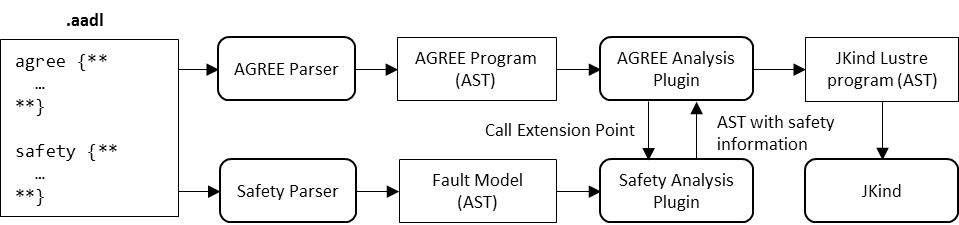
\includegraphics[trim=0 400 430 0,clip,width=0.85\textwidth]{images/arch.png}
		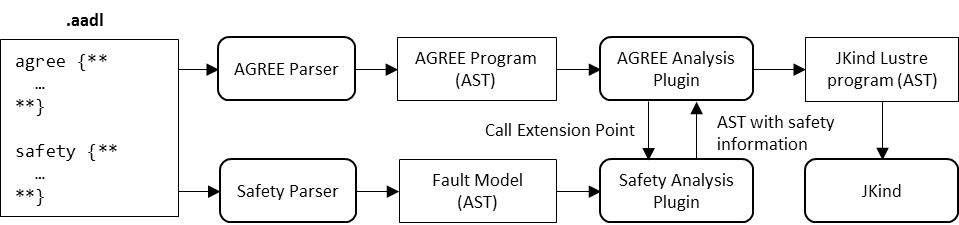
\includegraphics[width=\textwidth]{images/arch.png}
	\end{center}
	%\vspace{-0.1in}
	\caption{Safety Annex Plug-in Architecture}
	\label{fig:plugin-arch}
	%\vspace{-0.1in}
\end{figure}

\agree contracts are used to define the nominal behaviors of system components as guarantees that hold when assumptions about the values the component's environment are met. When an AADL model is annotated with \agree contracts and the fault model is created using the Safety Annex, the model is transformed through \agree into a \lustre model~\cite{Halbwachs91:IEEE} containing the behavioral extensions defined in the \agree contracts for each system component. 

When an AADL model is annotated with \agree contracts and the fault model is created using the Safety Annex, an extension point between \agree and the Safety Annex allows the fault information to be added to the \agree \textit{abstract syntax tree} (AST). This extended model AST is then translated into \lustre~\cite{Halbwachs91:IEEE}, a synchronous dataflow language used by \jkind, an infinite-state model checker for safety properties~\cite{2017arXiv171201222G}. 

The fault model extension of the contracts written in \agree allows faults to modify the behavior of component outputs. An example of a portion of a nominal \agree node written in \lustre and its extended contract is shown in Figure~\ref{fig:lustre}. The left column of the figure shows the nominal \lustre pump definition with an \agree contract on the output; and the right column shows the additional local variables for the fault (boxes 1 and 2), the assertion binding the fault value to the nominal value (boxes 3 and 4), and the fault node definition (box 5). Once augmented with fault information, the \agree model follows the standard translation path to the model checker \jkind. 

\begin{figure}[h!]
	\hspace*{-2cm}
	%\vspace{-0.1in} 
	\begin{center}
		%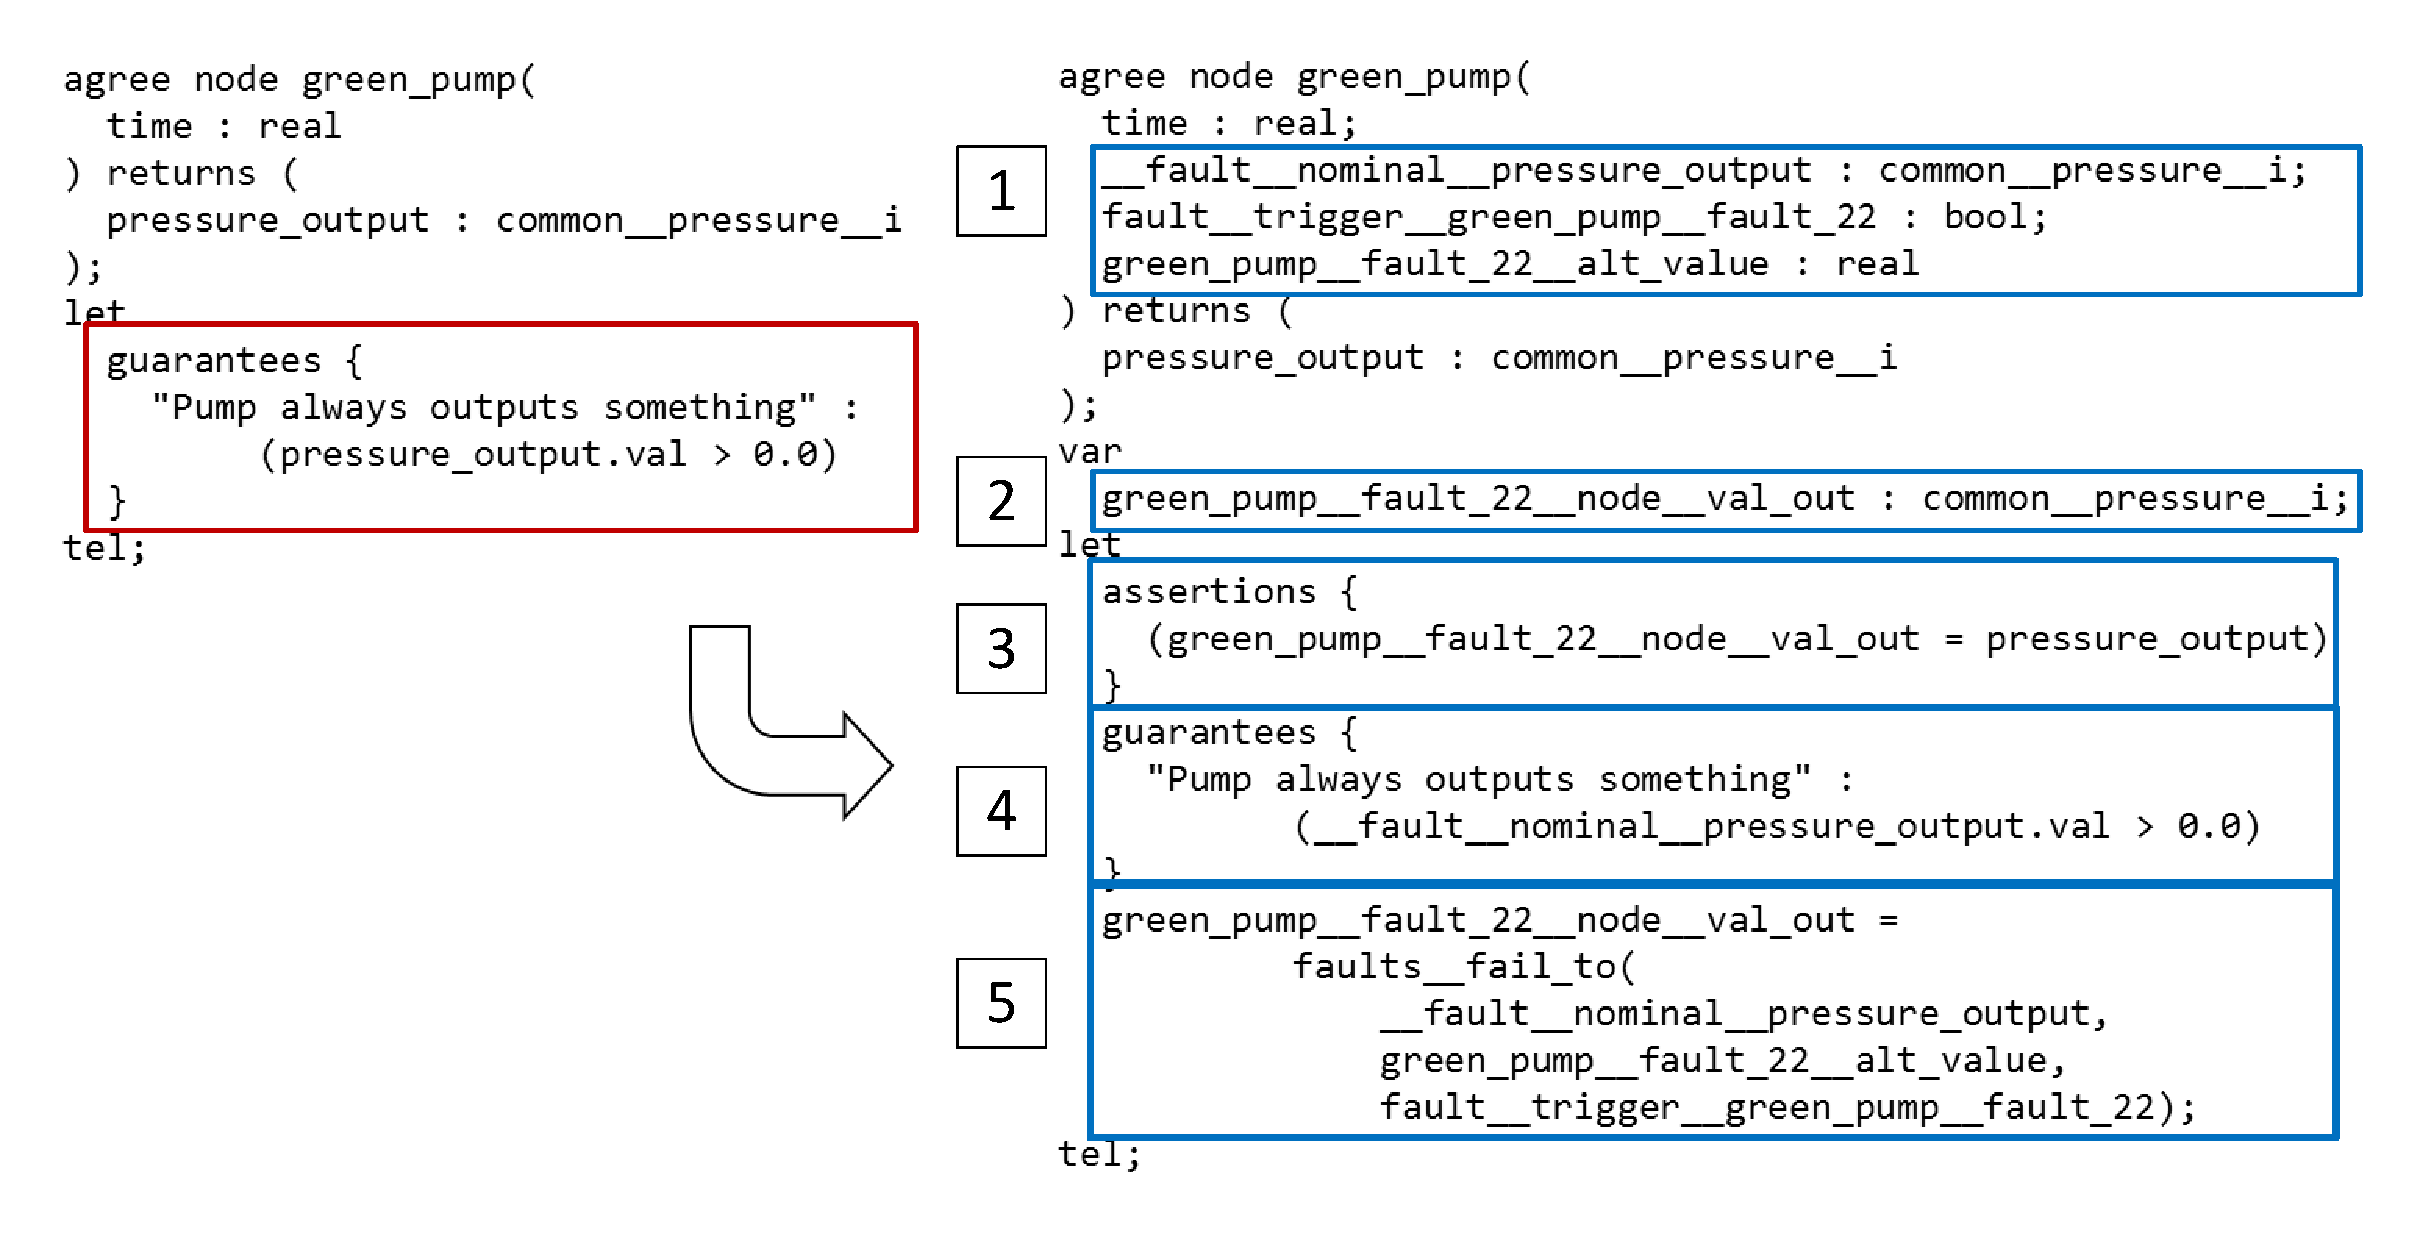
\includegraphics[trim=0 690 -10 70,clip,width=1.5\dimexpr\textwidth-2cm\relax]{images/lustre.pdf}
		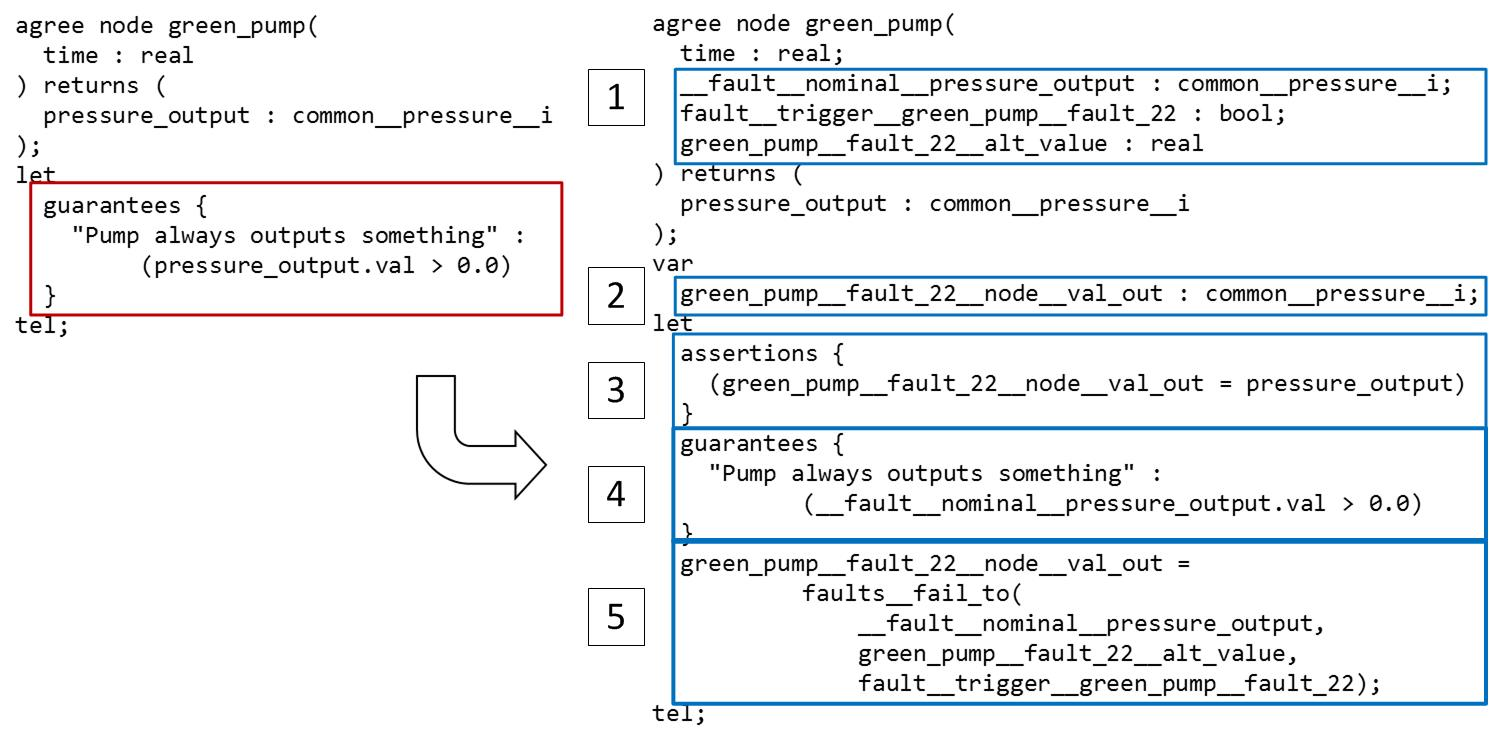
\includegraphics[scale=0.3]{images/lustre.jpg}
		%\caption{Nominal \agree node and its extension with faults}
		\caption{Nominal \agree Node and Extension with Faults}
		\label{fig:lustre}
	\end{center}
	%\vspace{-0.1in}
\end{figure}


\subsection{The Sensor System}
\label{sec:sensorExample}
An example is a helpful guide to illustrate the Safety Annex. A simple sensor system is shown in Figure~\ref{fig:sensorSys}. The top level of the system takes two inputs; environmental pressure and temperature. Each subsystem monitors its corresponding input and will send an shutdown command if the input surpasses some threshold. Each subsystem consists of three sensors. Each subsystem's output is regulated by a majority voter; thus, if the majority of sensors in a subsystem report high temperature (or pressure), the shutdown command is sent. 

\begin{figure}[h]
	%\vspace{-0.956in}
	\centering
	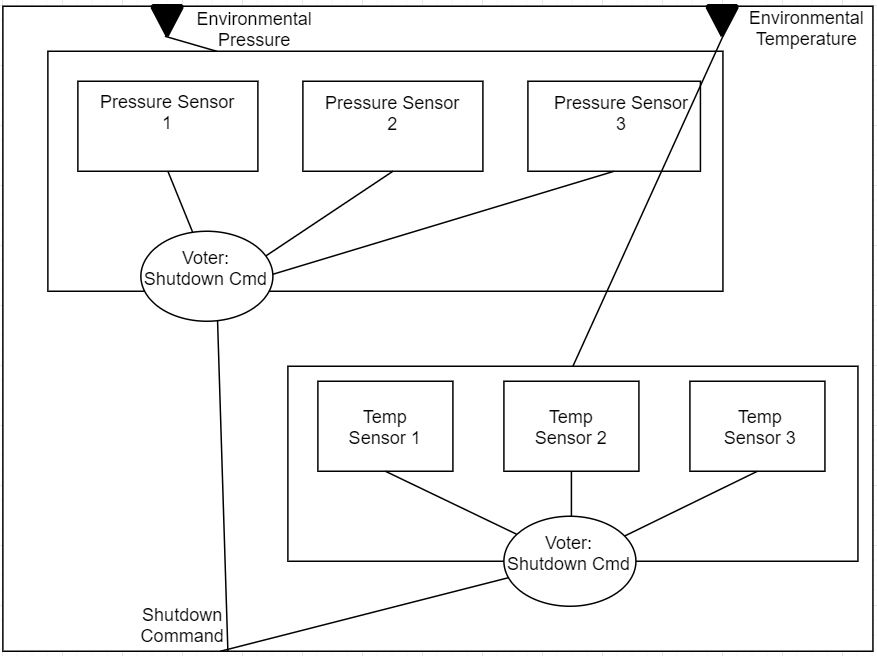
\includegraphics[width=0.6\textwidth]{images/two_sensors.PNG}
	%\vspace{-0.4in}
	\caption{A Simple Sensor System}
	\label{fig:sensorSys}
\end{figure}

This example will be referenced intermittently throughout this document.  

\subsection{The Safety Annex for the Sensor System}
In short, the Safety Annex allows users to describe faults and connect them to AADL component outputs. Within the AADL component instance model, an annex is added which contain the fault definitions for the given component. The flexibility of the fault definitions allows the user to define numerous types of fault \textit{nodes} by utilizing the \agree node syntax. An example of the \agree and Safety Annexes defined on a pressure sensor in the sensor system is shown in Figure~\ref{fig:annexes}. 
\begin{figure}[h]
	%\vspace{-0.956in}
	\centering
	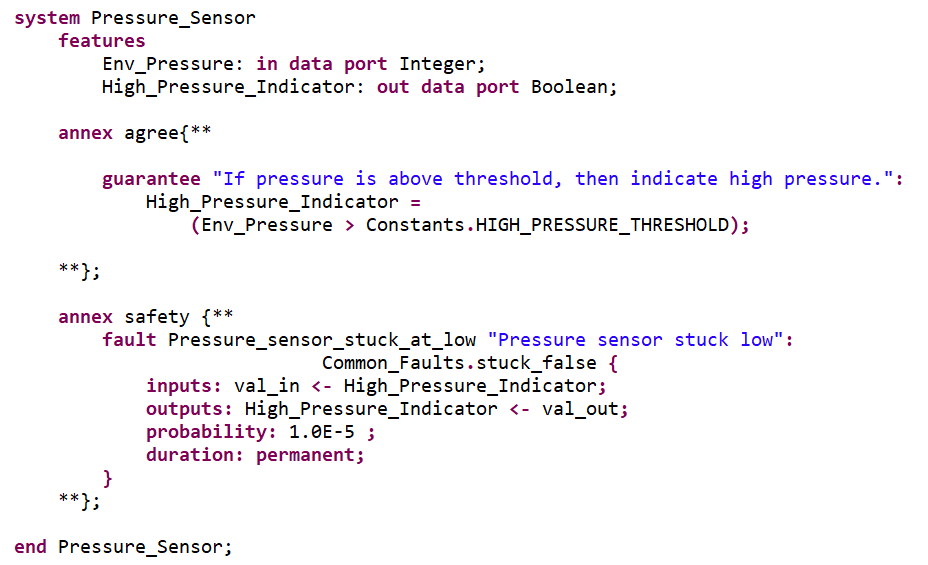
\includegraphics[width=0.7\textwidth]{images/sensorAnnexes.PNG}
	%\vspace{-0.4in}
	\caption{A Pressure Sensor and the \agree and Safety Annexes}
	\label{fig:annexes}
\end{figure}
The fault definition connects to a \textit{fault node} that is defined in Figure~\ref{fig:node} (the reference to this fault node is seen in the syntax of the fault definition in Figure~\ref{fig:annexes}: \texttt{Common\_Faults.stuck\_false}). The fault node, \texttt{stuck\_false}, restricts the output to false, even when the pressure is higher than the threshold.
\begin{figure}[h]
	%\vspace{-0.956in}
	\centering
	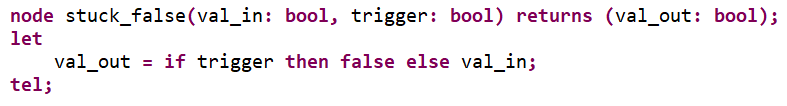
\includegraphics[width=0.6\textwidth]{images/sensorNode.PNG}
	%\vspace{-0.4in}
	\caption{A Fault Node Definition}
	\label{fig:node}
\end{figure}

When a fault is activated by a trigger condition, the fault node outputs a value which overrides the component's nominal output value. The faulty behavior may violate the contracts of other components in the system, including assumptions of downstream components. The impact of a fault is shown by counterexamples returned by the model checker when fault analysis is run on the model.

The fields of a fault definition are shown in Figure~\ref{fig:annexes} and are described for clarity.
\begin{itemize}
\item \textbf{Fault node statement}: This is seen as \texttt{Common\_Faults.stuck\_false} in the figure and refers to a file of fault node definitions (\texttt{Common\_Faults}) containing commonly used faults such as stuck false, stuck true, fail to, or in this case \texttt{stuck\_false}. This provides the node definition in the \lustre code.
\item \textbf{Input}: The inputs state which values from the component are passed into the node definition. In this case, the nominal component (pressure sensor) output \texttt{High\_Pressure\_Indicator} is passed into the node parameter \texttt{val\_in}. 
\item \textbf{Output}: The output from the fault node is designated to an AADL component feature, essentially overwriting it if the fault is active. In this case, the node's output will be the pressure sensor output: \textit{High\_Pressure\_Indicator}. 
\item \textbf{Probability}: This field specifies the probability of occurrence for this fault. This is required for probabilistic analysis.
\item \textbf{Duration}: When a fault becomes active, it is designated as a permanent fault. 
\end{itemize}

\subsection{Modeling Dependent Faults}
%Within the AADL component instance model, the Safety Annex is added which contain the fault definitions for the given component. When a fault is activated by its specified triggering conditions, it modifies the output of the component. This faulty behavior may violate the contracts of other components in the system, including assumptions of downstream components. 
The impact of a fault is computed by the \agree model checker when the safety analysis is run on the fault model and thus determined implicitly; the error propagation is not explicitly defined as in other closely related tools~\cite{EMV2,compass30toolset}. However, failures in hardware (HW) components can trigger behavioral faults in the system components that depend on them. This makes it beneficial to allow for explicit error propagation and the notion of dependencies in the fault model. For example, a CPU failure may trigger faulty behavior in the threads bound to that CPU or a failure in one HW component may trigger failure in other HW components located nearby, such as overheating, fire, or an explosion in the containment location. The Safety Annex provides the capability to explicitly model the impact of hardware failures on other faults, behavioral or non behavioral. 

Users specify dependencies between the HW component faults and faults that are defined in other components, either HW or SW. The hardware fault then acts as a trigger for its dependencies. This allows for propagation from the faulty HW component to the components that rely on it, affecting the behavior on the outputs of the affected SW components. Within the \lustre implementation, this corresponds to a statement linking the active fault to all dependent faults. Thus, if the triggering fault is active, so are all dependencies.

\section{Verification Capabilities in the Face of Component Failures}
When performing safety analysis, it is useful to be able to restrict the number of failed components in terms of a maximum number or a probabilistic computation. Instead of allowing the \lustre fault activation assignments to remain unrestricted, statements can be added to the Safety Annex that specify the type of analysis to be run. This is either \textit{maximum fault analysis} or \textit{probabilistic threshold analysis}. 

The fault analysis statement (also referred to as the fault hypothesis) resides in the AADL system implementation that is selected for verification. This may specify either a maximum number of faults that can be active at any point in execution (Figure~\ref{fig:hypothesisMaxN}) or that the only faults to be considered are those whose probability of simultaneous occurrence is above some probability threshold (Figure~\ref{fig:hypothesisProb}).

\begin{figure}[h!]
	\vspace{-0.1in}
	\begin{center}
		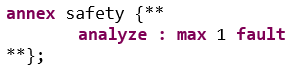
\includegraphics[width=0.4\textwidth]{images/hypothesisMaxN.png}
	\end{center}
	\vspace{-0.1in}
	\caption{Max N Faults Analysis Statement}
	\label{fig:hypothesisMaxN}
\end{figure} 

\begin{figure}[h!]
	\vspace{-0.1in}
	\begin{center}
		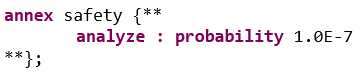
\includegraphics[width=0.5\textwidth]{images/hypothesisProb.png}
	\end{center}
	\vspace{-0.1in}
	\caption{Probability Analysis Statement}
	\label{fig:hypothesisProb}
\end{figure}

Tying back to the fault tree analysis in traditional safety analysis, the former is analogous to restricting the minimal cut sets to a specified maximum number of terms, and the latter is analogous to restricting the minimal cut sets to only those whose probability is above some set value. In the former case, we assert that the sum of the active faults is at or below some integer threshold.  In the latter, we determine all combinations of faults whose probabilities are above the specified probability threshold, and describe this as a proposition over fault activation literals. 
%
Active faults are divided into two categories: independently active (activated by its own triggering event) and dependently active (activated when the faults they depend on become active). The top level fault hypothesis applies to independently active faults. Faulty behaviors augment nominal behaviors whenever their corresponding faults are active (either independently active or dependently active).

\subsection{Maximum Fault Analysis}
The max fault hypothesis specifies a maximum number of faults that can be active at any point in execution. This is analogous to restricting the minimal cut sets to a specified maximum number of terms in the fault tree analysis in traditional safety analysis. In implementation (i.e., the translated \lustre model feeding into the model checker), we assert that the sum of the fault activation literals assigned to \textit{true} is below some integer threshold. This can be seen in Figure~\ref{fig:count} with maximum fault count set at 3.
\begin{figure}[h]
	%\vspace{-0.1in}
	\begin{center}
		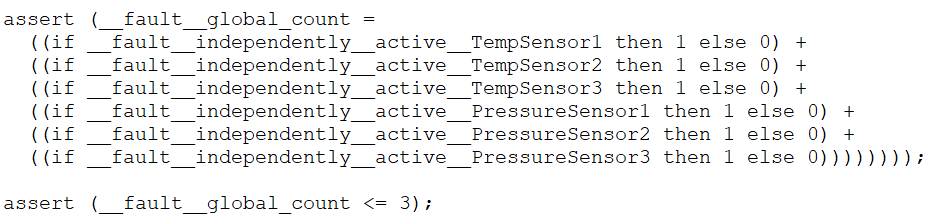
\includegraphics[width=0.7\textwidth]{images/assertCount.PNG}
	\end{center}
	%\vspace{-0.1in}
	\caption{\lustre Statement for Fault Count}
	\label{fig:count}
\end{figure}
While solving the satisfiability problem, JKind will iterate through the possible combinations given the restriction of the hypothesis statement. If the system with respect to a certain safety property is found to be UNSAT, a counterexample showing the trace of the system (including active faults) is given to the user. 

When running the analysis compositionally, JKind employs a top-down approach; it attempts to prove the top-level requirements using the contracts of the direct subcomponents, then it moves to the next layer down, and so on. If using maximum N fault analysis compositionally, the results pertain only to the current level of analysis.

In the traditional safety assessment process, safety analysts require information regarding single points of failure on specific components or even system wide. The Safety Annex supports this need and the detailed counterexamples can provide important insight into the system development process. 

\subsection{Probabilistic Threshold Analysis}
The grammar of the Safety Annex allows for a probabilistic assignment to a fault definition as shown in Figure~\ref{fig:annexes}. The \textit{probabilistic fault hypothesis} specifies that only faults whose probability of simultaneous occurrence is above some probability threshold should be considered. In the implementation, we determine all combinations of faults whose probabilities are above the specified probability threshold and describe this as a proposition over the fault activation literals. If the probability of a combination of faults is less than the designated top level threshold, these faults may be activated and the behavioral effects can be seen through a counterexample.  

To perform this analysis, it is assumed that the faults occur independently. Algorithm 1 describes this process. First, all faults are removed from consideration that are too unlikely given the probability threshold. The remaining faults are arranged in a priority queue $\mathcal{Q}$ from high to low. Take the fault with highest probability from the queue (step 5) and attempt to combine the remainder of the faults in $\mathcal{R}$ (step 7). If this combination is lower than the threshold (step 8), then we do not take into consideration this set of faults and instead remove the tail of the remaining faults in $\mathcal{R}$. %The reason we can do this is because of the arrangement in priority queue from highest to lowest value. If this combination is below threshold, certainly any other combination of these faults with one of lesser value in the priority queue will also be below threshold. 
 
In this calculation, we assume independence among the faults, but in the Safety Annex it is possible to define dependence between faults using a fault propagation statement. After the possible fault combinations are computed using Algorithm 1, the triggered dependent faults are added to the combination as appropriate while ignoring their respective probabilities.

\begin{algorithm}[H]
	% \KwData{this text}
	% \KwResult{how to write algorithm with \LaTeX2e }
	$\mathcal{F} = \{\}$ : fault combinations above threshold \;
	$\mathcal{Q}$ : faults, $q_i$, arranged with probability high to low \;
	$\mathcal{R} = \mathcal{Q}$ , with $r \in \mathcal{R}$\;
	\While{$\mathcal{Q} \neq \{\} \land \mathcal{R} \neq \{\}$ }{
		$q =$ removePriorityElement($\mathcal{Q}$) \;
		\For{$i=0:|\mathcal{R}|$}{
			$prob = q \times r_i$ \;
			\eIf{prob $<$ threshold}{
				removeTail($\mathcal{R}, i:|\mathcal{R}|$)\;
			}{
				add($\{q, r_i\}, \mathcal{Q}$)\;
				add($\{q, r_i\}, \mathcal{F}$)\;
			} % end if else
		} % end for
	} % end while
	\caption{Monolithic Probability Analysis}
\end{algorithm}

Often it is the case that safety properties contain probabilistic thresholds that must be analyzed during the safety assessment process. This type of fault hypothesis statement and the associated fault analysis supports these requirements.

\section{Generation of Minimal Cut Sets from MIVCs}
%\subsection{The General Idea}
As was previously explained, the MIVCs (Minimal Inductive Validity Cores) are \textit{MUS}s (Minimal Unsatisfiable Subsets) of a constraint system. The \textit{MCS}s (Minimal Correction Sets) can be obtained from all \textit{MUS}s by generating the hitting sets of all \textit{MUS}s. Thus, the \aivcalg algorithm produces all \textit{MUS}s and the hitting set algorithm can transform these into \textit{MCS}s. If the constraint system is defined to take into account faults, these \textit{MCS}s can be transformed into \textit{MinCutSets}. 

Recall that a constraint system is an ordered set of abstract constraints over a set of variables. In the case of a nominal model augmented with faults, a constraint system can be defined as follows. Let $F$ be the set of fault activation literals and $G$ be the set of component contracts (guarantees). 

\begin{definition}A constraint system $C = \{C_1,C_2,...,C_n\}$ where for $i \in \{1,...,n\}$, $C_i$ has the following constraints for any $f_j \in F$ and $g_k \in G$ with regard to the top level property $P$: 
\begin{center}
$C_i \in \left\{ \begin{array}{ll}
	f_j :&  false\\
	g_k :& true\\
	P :& false\\
\end{array}\right.$	
\end{center}
\label{def:constraintsystem}
\end{definition}

The \aivcalg algorithm collects all minimal unsatisfiable subsets of a given transition system in terms of the \textit{negation} of the top level property~\cite{Ghassabani2017EfficientGO,bendik2018online}. Assuming that the nominal model proves (no faults are active), it is not surprising that the guarantees (constrained to \textit{true}) and the negation of the safety property is UNSAT. The \textit{MUS}s are the minimal explanation of the infeasibility of this constraint system; equivalently, these are the minimal sets of model elements necessary for proof of the safety property.

We utilize this algorithm by providing not only component contracts constrained to \textit{true} as model elements, but also fault activation literals constrained to \textit{false}, i.e. the faults are inactive. Thus the resulting MIVCs (\textit{MUS}s) will contain the required contracts and constrained fault activation literals necessary to prove the safety property. 

Because of the duality between \textit{MUS}s and \textit{MCS}s, all \textit{MCS}s can be obtained by finding the hitting sets. The \textit{MCS} can be seen to correct the infeasibility of the constraint system and provides the minimal such correction. By removing the constraints from $C$ that are found in any \textit{MCS}, $C$ becomes satisfiable. In terms of our constraint system with fault activation literals, by \textit{activating} the faults in the \textit{MCS} and \textit{violating} the contracts in the \textit{MCS}, we can prove the \textit{negation} of the property $P$. If the contracts in the \textit{MCS} are replaced with the faults that cause its violation, the \textit{MCS} is transformed into a \textit{MinCutSet}.\\

\textbf{The Steps of Transformation from \textit{MUS} to \textit{MinCutSet}}
\begin{enumerate}
\item Redefine constraint system by adding fault activation literals to the constraint system used by the \aivcalg algorithm. %The MIVC algorithm proceeds compositionally, so the changes to the constraint system must also be factored in on a per-layer basis. For the leaf levels of the system, we add all fault activation literals as model elements for consideration. For all other layers, we provide the guarantees of the layer beneath and if the layer beneath is 
\item Transform the \textit{MUS}s (MIVCs) into \textit{MCS}s by use of a hitting set algorithm~\cite{murakami2013efficient,gainer2017minimal}. 
\item Replace all contracts in the \textit{MCS}s by the faults that cause their violation (\textit{MinCutSets} for that contract). 
\end{enumerate}

\subsection{Illustrative Example}
Using the sensor system described in Section~\ref{sec:sensorExample}, this transformation can be more easily understood. The top-level safety property of the system states that a shutdown occurs when and only when it should: 
\begin{center}
    ($temp\_input > threshold$) $\lor$ ($pressure\_input > threshold$)\\
    $\iff Shutdown$
    
\end{center}

The property of each sensor subsystem states that when the majority of sensors report high, denoted as $out_{si}$ for sensor $si$, a shutdown command is sent:
\begin{center}
    $majority\_vote(out_{s1}, out_{s2}, out_{s3}) \iff Shutdown$
    
\end{center}

Each sensor has a behavioral property stating that if the environmental input is high, the shutdown command is sent: 
\begin{center}
    $(environment > threshold) \iff Shutdown$
    
\end{center}

A fault is defined on each of the sensors which when active, causes the sensors to fail low (the environmental input is high, but they do not send a shutdown command). It is easy to see that this system is resilient to a single fault anywhere due to the majority voting mechanism. \\

\textbf{Leaf Level}: To illustrate the \textit{MIVC} to \textit{MinCutSet} transformation, we start with a leaf level of the system: a pressure sensor, $p1$. (Note: The \aivcalg algorithm proceeds in a top-down fashion, but for clarification in the example, we look at the results in a bottom-up approach.)  In this layer, the \aivcalg algorithm treats the sensor guarantee, $g_{p1}$, as the property of interest:
\begin{center}
    $g_{p1} : (environment > threshold) \iff Shutdown$
\end{center}
and the model elements provided to the \aivcalg algorithm consist of only fault activation literals for this leaf component constrained to \textit{false}; we call the fault on $p1$, $f_{p1}$. Thus, the constraint system for this layer is: 
\begin{center}
    $C_{leaf} = \{\neg f_{p1} \neg g_{p1}\}$
\end{center}

The \aivcalg algorithm returns all \textit{MIVC}s for this constraint system, $MIVC = \{\{\neg f_{p1}\}\}$, of which there is only one: in order for this leaf level guarantee to hold, the fault must be constrained to false. 

The hitting set algorithm finds that the set $\{\neg f_{p1}\}$ sufficiently 'hits' all \textit{MIVC}s and this is our \textit{MCS}. This means that if the constraint is removed from $f_{p1}$ in $C$, our constraint system is satisfiable. Thus, the \textit{MinCutSet} for $\neg g_{p1}$ is $\{f_{p1}\}$, and in the same manner, we find the \textit{MinCutSets} for $g_{p2}, g_{p3}$ and the guarantees for the temperature sensors. \\

\textbf{Mid Level}: For the mid-level pressure system, $P$, the guarantee of interest is: 
\begin{center}
    $g_P : majority\_vote(out_{p1}, out_{p2}, out_{p3}) \iff Shutdown$
\end{center}
and can be also written as: 
\begin{center}
    $g_P: ((out_{p1} \land out_{p2}) \lor (out_{p1} \land out_{p3}) \lor (out_{p2} \land out_{p3})) \iff Shutdown$
\end{center}

The constraint system looks only at the supporting guarantees (one level below) and any fault literals in the current level. Thus, the constraint system is: 
\begin{center}
    $C = \{g_{p1}, g_{p2}, g_{p3}, \neg g_P\}$
\end{center}

The resulting \textit{MIVC}s are: $\{\{g_{p1}, g_{p2}\}, \{g_{p1}, g_{p3}\}, \{g_{p2}, g_{p3}\}\}$. If any pairwise combination of guarantees hold, then the property $g_P$ holds, i.e. the shutdown command is sent. The hitting set algorithm determines all sets whose intersection with all \textit{MIVC}s are nonempty. In this case, they are equivalent to the \textit{MIVC}s. 

Since \textit{MinCutSets} only contain faults, a replacement must be made between the guarantees found in the \textit{MCS}s and the faults that cause the violation of these guarantees. We know those faults due to the processing done at the leaf level; after replacement, we obtain the \textit{MinCutSets} for $\neg g_P$: $\{\{f_{p1}, f_{p2}\}, \{f_{p1}, f_{p3}\}, \{f_{p2}, f_{p3}\}\}$.\\

\textbf{Top Level}: The top level safety property is:\\ $SP : $  $(temp\_input > threshold)$ $\lor$ $(pressure\_input > threshold) \iff Shutdown$, and requires guarantees from both the temperature and pressure subsystems, $g_P$ and $g_T$ respectively. The resulting \textit{MIVC}s are: $\{\{g_P\}, \{g_T\}\}$. This is also equivalent (in this case) to the \textit{MCS}s generated through the hitting set algorithm. Replacement of these contracts with the faults that cause their violation produces all \textit{MinCutSets} for the top level event (violation of the top level safety property). This is: any combination of two faults occurring in either the temperature or the pressure sensor systems will result in violation of the safety property. 

\begin{figure}[h!]
	\centering
	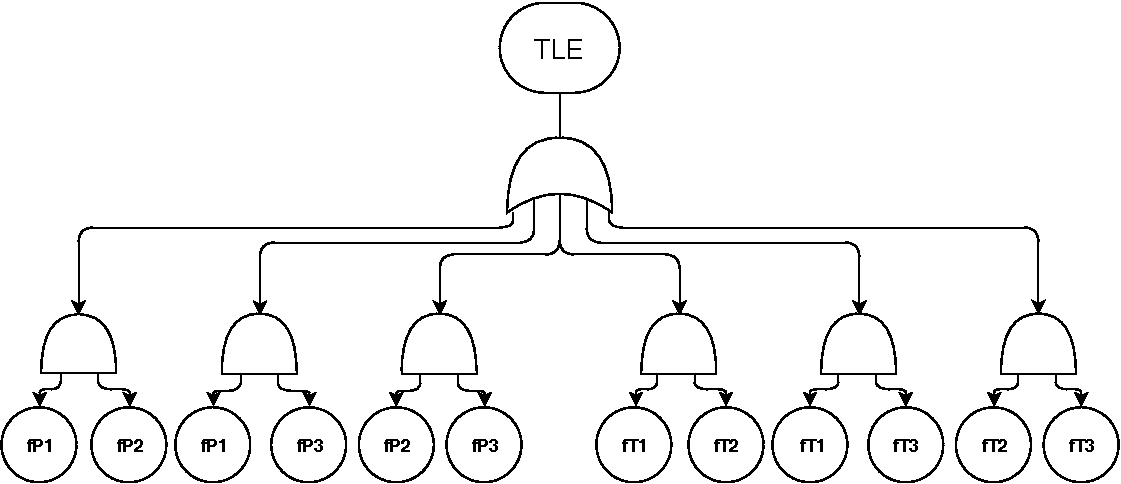
\includegraphics[trim=0 0 0 0,clip,width=0.85\textwidth]{images/flatFT.pdf}
	\caption{Flat Fault Tree for the Sensor Example}
	\label{fig:flatFT}
\end{figure}
\newpage
A typical fault tree generated by many of the current research tools available shows very little hierarchical information. An example of a flat fault tree is shown in Figure~\ref{fig:flatFT} and shows only the \textit{MinCutSets} that contribute to the top level event (TLE). (Note: probabilistic information is usually displayed with the fault tree, but not included here for readability.)

\begin{figure}[h!]
	\centering
	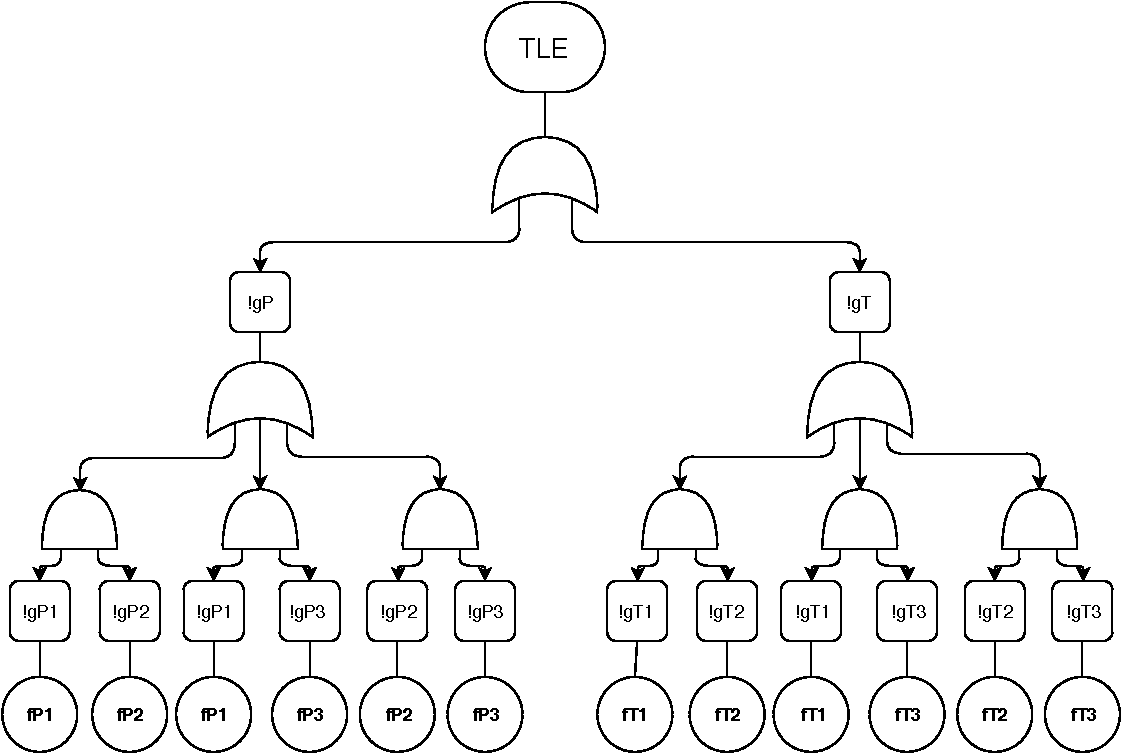
\includegraphics[trim=0 0 0 0,clip,width=0.85\textwidth]{images/ftSensor.pdf}
	\caption{Hierarchical Fault Tree for the Sensor Example}
	\label{fig:ftSensor}
\end{figure}

An example of a hierarchical fault tree that could be produced by the information gathered through this process is shown in Figure~\ref{fig:ftSensor}. Each layer of the architecture is shown in the fault tree and represented by the violated contracts of that layer. The OR-gate between the lower level contracts and the TLE reflects the safety property itself: if either of the subsystems fail, the safety property is violated. The second layer of the tree also reflects the relationship between the sensors and the sensor subsystem: if any pairwise combination of sensors fail, the mid-level contract is violated. This process of using \textit{IVC}s to generate minimal cut sets will provide layer by layer the necessary information to not only collect the \textit{MinCutSets}, but also reflect the hierarchical nature of the system within the fault trees generated.

The example should suffice to show the basic outline of the algorithm. The proofs showing that this transformation is logically valid will be provided in the dissertation and the algorithms will be implemented in the Safety Annex.  


\section{Compositional Probabilistic Computations}
Safety analysis techniques aim at demonstrating that the system meets the requirements necessary for certification and use in the presence of faults. In many domains, there are two main steps to this process: (1) the generation of all minimal cut sets (\textit{MinCutSets}), i.e. the minimal set of faults that lead to a violation of the top level property (known as a \textit{top-level event} or TLE) and (2) the computation of the corresponding fault probability, i.e. the probability of reaching the TLE, given probabilities for the faults in the system. 

The probability of the TLE is used to find the likelihood of the safety hazard that it represents. While evaluation of the fault model with a given probabilistic threshold does provide information on the safety hazards, it is also informative and desirable to find the overall probability of the occurrence of a hazard. 

Such computations can be carried out by leveraging the logical formula represented by the disjunction of all \textit{MinCutSets} which are in turn conjunctions of their constituents. 

Given a set of \textit{MinCutSets} and a mapping $\mathcal{P}$ that gives the probability of the basic faults in the system $f_i$, it is possible to compute the probability of occurrence of the TLE. Assuming that the basic faults are independent, the probability of a single \textit{MinCutSet}, $\sigma$ is given by the product of the probabilities of its basic faults:
\begin{center}
    \begin{equation*}\mathcal{P}(\sigma) = \prod_{f_i \in \sigma} \mathcal{P}(f_i) 
    \end{equation*}    
\end{center}

For a set of \textit{MinCutSets}, $S$, the probability can be computed using the following recursive formula:

\begin{center}
    $\mathcal{P}(S_1 \cup S_2) = \mathcal{P}(S_1) + \mathcal{P}(S_2) - \mathcal{P}(S_1 \cap S_2)$
\end{center}

Due to the independence assumption, $\mathcal{P}(S_1 \cap S_2)$ is computed as $\mathcal{P}(S_1) \cdot   \mathcal{P}(S_2)$. Using this technique, it is theoretically possible to compute the overall probability of a TLE given all \textit{MinCutSets} and an independence assumption, but in the real world of safety analysis this poses some problems, the largest of which is scalability. Given a very large system with many possible faults, it becomes difficult to compute all \textit{MinCutSets} without pruning of any kind. If one is unable to complete such computations, it is not possible to simply compute the probabilities as described above. 

As previously discussed, it is standard practice to consider cut sets only up to a given cardinality. As the cardinality of the cut sets increase, the likelihood of their occurrence decreases and as the system increases in size, the possible combinations of problematic faults will inevitably increase, at times exponentially. In order to simplify these calculations and address the problem of scalability, \textit{MinCutSets} up to a certain cardiality are considered. Everything above that is "safely" ignored, and then specific criteria is used to over-approximate the error. The end result of these computations is above the actual probability (i.e. a safe approximation), but close enough to be significant. 

Another drawback to computing an exact probability of the TLE is the problem of model reliability and exactness. For instance, if two groups of engineers each built a model of the same system, the models may not be equivalent; especially in terms of behavioral properties. Since our approach of computing \textit{MinCutSets} depends on the properties over system components, the calculated top-level probability will change. Different representations of the system will alter the computations.  

As an example, assume that Figure~\ref{fig:probComp1} is a snapshot of a given layer in a system designed by the first group of engineers. Component A has a contract, $G_A$, which is determined by the \aivcalg algorithm to depend on a lower level contract, $g_A = a \land b$. $g_A$ will be in the set of \textit{IVC}s for the contract $G_A$. Assume that only $a$ is required for the proof of $G_A$. 

\begin{figure}[h]
\begin{center}
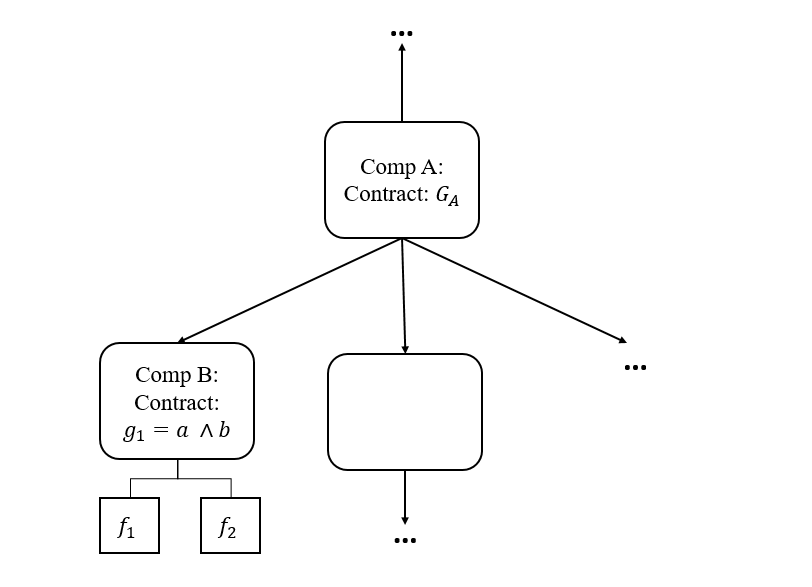
\includegraphics[width=6cm]{images/probComp1.PNG}
\caption{Sample System Contract Part I} \label{fig:probComp1}
\end{center}
\end{figure}

Two faults are defined on component B: $f_1$ violates $a$ and $f_2$ violates $b$. Since each of these faults will violate the contract $g_A$, each of these faults will be found in \textit{MinCutSets} for $G_A$.

Now assume that Figure~\ref{fig:probComp2} was the system representation built by the second group of engineers. 
\begin{figure}[h]
\begin{center}
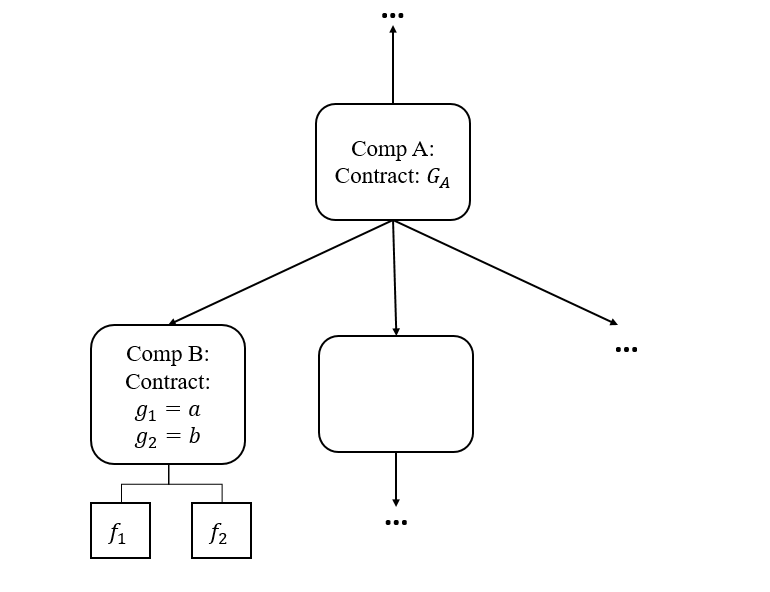
\includegraphics[width=6cm]{images/probComp2.PNG}
\caption{Sample System Contract Part II} \label{fig:probComp2}
\end{center}
\end{figure} 
The basic system structure is the same, but this time there are two contracts for component B: $g_1 = a$ and $g_2 = b$. Since $b$ is not required for the proof of $G_A$, only $g_1$ is found in the \textit{IVC}s for $G_A$ and thus only $f_1$ will be seen in the \textit{MinCutSets} for this particular contract. 

In this simple example, it is easy to see why a single computation of the top-level probability of a system may be misleading and may not reflect the actual probability of the system. To this end, we wish to find a way to accurately obtain higher and lower bounds of what the probability is likely to be. 

A lower bound for the probability can be obtained by choosing a maximum cardinality for \textit{MinCutSets} before computations begin, e.g. assume that cardinalities above $n$ are too unlikely to be significant. This will contribute to better scalability in large systems with numerous possible cut sets. A higher bound is commonly assigned by experts of the system, e.g. around 3 orders of magnitude higher than the lower approximation. 

It would be beneficial to leverage the \textit{IVC} information to provide both the lower and upper bound approximations and show that these values are significant and trustworthy. 



\section{Evaluation of Results}
The goal of this dissertation is to provide usable and reliable safety assessment artifacts and methodologies that can be implemented on industrial scale systems. Furthermore, the artifacts should shed light on the system organizational hierarchy, interacting components, and problematic faults. This is useful within the assessment process and can provide valuable feedback to engineers on both the safety and development side. 

To this end, we will implement a large scale system model in the aerospace domain and collect the artifacts and other pertinent information derived from this process. We will show how this information can provide feedback to the system engineers and be useful in the certification process. 

The Wheel Brake System (WBS) was initially developed for illustrative purposes by SAE AIR6110~\cite{AIR6110} and has been used in numerous case studies and research into Model-Based Safety Analysis~\cite{Stewart17:IMBSA,DBLP:conf/cav/BozzanoCPJKPRT15,mcmillan2019increasing,cimatti2016temporal,cimatti2018tightening,konrad2016faa}. This model is large enough to assess scalability and provides numerous complex component interactions and behaviors. The AADL version of this model will be annotated with \agree contracts that accurately describe the behavior of the system components. Faults will be attached to each of the components as per descriptions in AIR6110. The analysis of this approach will address the four main contributions of the Safety Annex: 
\begin{enumerate}
    \item Maximum $n$ fault threshold compositional analysis
    \item Probabilistic threshold monolithic analysis 
    \item Minimal cut set computations (max $n$ and probabilistic threshold)
    \item Probabilistic evaluations and computations
\end{enumerate}

The artifacts generated from each run will be assessed in light of safety assessment and fit into the process as described in Sections \ref{sec:saProcess} and \ref{sec:saProcess2}.

Using other models representative of the aerospace industry, we will explore the necessity of using a shared system model that drives the development and safety processes, and show the fault modeling flexibility of the Safety Annex. 











 % The four contributions
\chapter{Conclusion}
\label{chap:conclusion}
System safety analysis is crucial in the development of critical systems and the generation of accurate and useful results is invaluable to the assessment process. Having multiple ways to capture complex dependencies between faults and the behavior of the system in the presence of these faults is important throughout the development process. A model-based approach was proposed that allows for a tighter integration between system development and safety analysis. The existing system model is extended and safety specific definitions and information can be defined at all levels of the model architecture (e.g., software, hardware, system level, module level). This extended model, or fault model, can be analyzed using a model checker and various safety related artifacts can be generated. These include snapshots of the state of the system when a fault is active (automatically generated counterexamples), maximum active fault thresholds, and minimal cut sets. 

We also provided a formalization of the compositional generation of minimal cut sets through the use of inductive validity cores. This will open the door for future research work into more scalable options of minimal cut set generation through the use of SMT-solvers and possibly other verification engines. 

An introductory exploration into the concepts of granularity and mutation testing provides a framework for the application of other kinds of formal methods techniques on a fault model and what kinds of important information can be gleaned from such analyses. 

All of this contributes to the \textbf{long range goal of the research}: to increase system safety through the support of MBSA process backed by formal methods to help safety engineers with early detection of design issues and automation of the artifacts required for certification.  % Summary of contributions

% \printglossary[title={LIST OF TERMS}, toctitle={List of Terms}]

%%%%%%%%%%%%%%%%%%%%%%%%%%%%%%%%%%%%%%%%%%%%%%%%%%%%%%%%%%%%%%%%%%%%%%%%%%%%%%%%
% WORKS CITED
%%%%%%%%%%%%%%%%%%%%%%%%%%%%%%%%%%%%%%%%%%%%%%%%%%%%%%%%%%%%%%%%%%%%%%%%%%%%%%%%
% When you need a works cited section, uncomment this and update the name of the
%   file.
%%%
    \bibliographystyle{abbrv}
%     \bibliographystyle{abbrvnat}
\bibliography{noAbbreviations,biblio}


%%%%%%%%%%%%%%%%%%%%%%%%%%%%%%%%%%%%%%%%%%%%%%%%%%%%%%%%%%%%%%%%%%%%%%%%%%%%%%%%
% APPENDICIES
%%%%%%%%%%%%%%%%%%%%%%%%%%%%%%%%%%%%%%%%%%%%%%%%%%%%%%%%%%%%%%%%%%%%%%%%%%%%%%%%
% If you need an appendix, uncomment the following lines and add sections.
%%%
%\appendix
%\input{sectionName}

\end{document}
